\documentclass[french,10pt]{article}
\usepackage[T1]{fontenc}
\usepackage[utf8]{inputenc}
\usepackage{lmodern}
\usepackage[a4paper,top=1.0cm, left=1.0cm, right = 1.0cm, bottom = 1.2cm]{geometry}
\usepackage{amsmath}
\usepackage{tikz}
\usepackage{pgfplots}
\usepackage{subfig}

\def\spaceans{\underline{\hspace{1cm}}}
\def\spaceTF{$\big(\quad\big)$}



\title{ \large
	Faculté de Sciences et Technologie - UPEC \\
	$2^{\textrm{éme}}$ Contrôle Continu de Mécanique du Point 1 (29/11/2023)\\ }
\author{Responsable TD: Felipe FIGUEREDO ROCHA \\ \texttt{felipe.figueredo-rocha@u-pec.fr}}

\date{}
\begin{document}
	
	\maketitle
	
	\thispagestyle{empty}
	
	\vspace{-0.5cm}
	NOM:\underline{\hspace{7cm}} Prénom: \underline{\hspace{5cm}}  Numéro: \underline{\hspace{2cm}} \\
	Licence:\underline{\hspace{7cm}} Groupe: \underline{\hspace{5cm}} Note: \underline{\hspace{1.5cm}}

	\subsection*{Instructions et rappels}
	\begin{itemize}
		\item Calculettes et téléphones portables interdits (stricte! le nom sera remonté aux coordinateurs). 
		\item N'oubliez pas les unités, des flèches au-dessus des vecteurs, etc.
		\item On négligera la poussé d'Archimède et le frottement sauf si autrement dit.
	\end{itemize}
	
	\begin{itemize}
		\item Dérivé d'un fonction composé: $(f \circ g)'(x) = (f' \circ g)(x) g'(x)$.
		\item Produit scalaire en deux dimensions : $\vec{a} \cdot \vec{b} = a_x b_x + a_y b_y = \|a\| \|b\| \cos{\theta}$, où $\theta$ est l'angle entre $\vec{a}$ et $\vec{b}$.
		\item Quelques relations en repère polaire avec l'angle $\theta$ mesuré par rapport $\Vec{u}_x$ (ci-dessous dépendance explicite du temps omis, $r=r(t) , \theta=\theta(t), \Vec{u}_r = \Vec{u}_r(t), \Vec{u}_{\theta} = \Vec{u}_{\theta}(t)$):
		\begin{align*}
			\Vec{u}_r &= \cos{\theta} \Vec{u}_x + \sin{\theta} \Vec{u}_y, \quad \Vec{u}_{\theta} = -\sin{\theta} \Vec{u}_x + \cos{\theta} \Vec{u}_y, \quad, 
			\dot{\Vec{u}}_r = \dot{\theta} \Vec{u}_{\theta}, \quad  \dot{\Vec{u}}_{\theta} = -\dot{\theta} \Vec{u}_{r}, \\
			\vec{OM}(t) &= r \vec{u}_r, \quad  d\vec{OM}(t) = d r \vec{u}_r + r d\theta \vec{u}_{\theta}, \quad
			\Vec{v}(t) = \dot{r} \Vec{u}_r + r \dot{\theta} \Vec{u}_{\theta}, \quad
			\Vec{a}(t) = (\ddot{r} - r\dot{\theta}^2) \Vec{u}_r + (2 \dot{r} \dot{\theta} + r \ddot{\theta}) \Vec{u}_{\theta}
		\end{align*}
		\item Travail d'une force entre $A$ et $B$ : $\displaystyle W_{A \to B}(\vec{F}) = \int_A^B \vec{F} \cdot d\vec{OM} $
		\item Enérgie cinétique en $A$ (instant $t_A$) : $E^A_c = \frac{1}{2} m \|\vec{v}(t_A)\|^2$ 
		\item Theorème d'énergie cinétique entre $A$ et $B$: $E_c^B - E_c^A = \sum_{\Vec{F}}  \displaystyle W_{A \to B}(\vec{F})$. 
	\end{itemize}
	
	\subsection*{Q1 (10 pts) : skateur dans un half-pipe (analogue pendule)}
	Un skateur de masse $m$ est sur un half-pipe semi-circulaire (moitié d'un cercle) de rayon $R$. On va considérer le skateur comme une particule M qui ne décolle jamais du half-pipe, c'est-à-dire, il sera toujours à une distance $R$ de l'origine $O$. On repère la position du skateur par l'angle $\theta$ qu'il fait avec la vertical descendent depuis $O$. La norme de l'accéleration de la pesanteur est dénoté $g$ (le vecteur $\Vec{g}$ pointe vers le bas). On va étudier ce mouvement en repère polaire.
	\begin{enumerate}
	\item Complétez la Figure 1 ci-dessous en plaçant $\theta$, $\Vec{u}_x$, $\Vec{u}_y$, $\Vec{u}_r$, $\Vec{u}_\theta$ selon la convention usuelle (voir rappel si besoin et notez qu'il de fléchés en plus).

	\begin{figure}
		\centering
		\includegraphics[width=0.5\linewidth]{halfpipe}
		\caption{}
		\label{fig:halfpipe}
	\end{figure}
	
	
	\item Faire un bilan de forces (sans frottement) appliqué sur la particule $M$ et donner les expressions de toutes les forces en repère polaire (n'oubliez pas de dessiner ces vecteurs).
	\item Donner les expressions simplifiés pour ce type de mouvement pour les vecteurs vitesse $\Vec{v}$ et accélération $\Vec{a}$ en repère polaire (voir rappel).
	\item Appliquer le principe fondamentale de la dynamique (PFD) et les projeter sur l'axe $\Vec{u}_{\theta}$ et $\Vec{u}_{r}$.
	\item En utilisant le PFD sur $\Vec{u}_{\theta}$, déduire l'équation différentiel qui gouverne ce mouvement en utilisant l'approximation $\sin \theta \approx \theta$ pour des petites oscillations.
	\item Vérifiez qu'une solution du type $\theta(t) = A \sin{\omega t}$ peut satisfaire l'équation précédent. Donner aussi l'expression pour $\omega$ en fonction de $g$ et $R$. 
	\item Dans l'instant initial le skateur est au tout au fond du half-pipe, avec $\theta(0) = 0$, et il imprime une vitesse angulaire (par exemple en s'autopropulsant avec ces pieds) de sorte que $\dot{\theta}(0) = \dot{\theta}_0$. Déterminez la constant $A$ en fonction de $\dot{\theta}_0$ et $\omega$. Qu'est-ce que représente $A$ et donner sa dimension. 
	
	\item Ce mouvement circulaire est-il uniforme ou non-uniforme? pourquoi? 
	\item Pour le cas particulier de $R = 10 \rm m$, $g = 10 \rm{m/s^2}$, $\dot{\theta}_0 = 5\times 10^{-2} \rm{rad/s}$, calculer $\omega$ et $A$.
	
	\item Pour ce cas particulier, tracer $\theta(t)$ pour $t \in [0 \rm s,T]$, où $T$ est temps nécessaire pour que la fonction sinus complète son cycle. N'oubliez pas de calculer $T$ (en fonction de $\pi$) et d'écrire la valeur de $T$ et $A$ sur le dessin. 
		\thispagestyle{empty}
	\begin{tikzpicture}
		\begin{axis}[
			%		xmin=-0.2, xmax=4, ymin=-0.2, ymax=3, 
			axis x line=middle, 
			axis y line=middle, 
			xlabel = {$t$},
			ylabel = {$\theta(t)$},
			ymajorgrids=true,
			xmajorgrids=true,
			grid style=dashed,
			xmin=-0.2,xmax=4.5,
			ymin=-1.5,ymax=1.5,
			xtick={1,2,3,4},
			xticklabels={$T/4$,$T/2$,$3T/4$,$T$},
			ytick={-1,0,1},
			yticklabels={$$, $$}
			]	
		\end{axis}
	\end{tikzpicture}

	\item Donner l'expression d'énérgie cinétique générique en fonction de $R$, $m$ et $\dot{\theta}$ (utilisez la formule de vitesse du l'exercise 3). 
	\item Pour le cas particulier l'exercise 9 et pour $m=80 \rm kg$, calculer l'énergie cinétique du skateur de masse  à l'instant $t=0 \rm s$. 
	\item Donner l'expression du travail $W_{0\to f}(\Vec{P})$ réalisé par la force de poids entre $\theta_0 = 0 \, \rm rad$ et $\theta_f$, en fonction des valeurs génériques de $m, g, \theta_f$.
	\item En utilisant le théorème d'énergie cinétique, donner l'expression pour $\dot{\theta}_{0}$ nécessaire pour que le skateur arrive jusqu'au bord supérieur du half-pipe (à $\theta_f = \pi/2$) mais sans le dépasser. 
	\item Maintenant, une force de frottement constant est présent $\Vec{f} = -f \Vec{u}_{\theta}$ (en supposant $\dot{\theta}_{0}$ > 0), donner une expression $\dot{\theta}_{0}$ sous les mêmes conditions du problème précédent.  
	\end{enumerate}
		
	\subsection*{Q2 (6 pts) : repère polaire alternatif }
		Imaginons que dans une autre pays du monde la convention préféré pour le repère polaire est tel que la position d'une particule $M$ soit paramétrisé par sa distance $\rho = \rho(t)$ (variable avec le temps) par rapport l'origine $O$ et une angle $\alpha = \alpha(t)$ (variable avec le temps) mesuré par rapport à $\Vec{u}_y$ de tel sorte que $\Vec{e}_{\rho} = -\sin{\alpha} \Vec{u}_x + \cos{\alpha} \Vec{u}_y$ et $\Vec{e}_{\alpha} = \cos{\alpha} \Vec{u}_x + \sin{\alpha} \Vec{u}_y$ représente les vecteurs radiale et circonférentielle de la base, respectivement (notez qu'on a utilisé d'autres lettres pour cette nouvelle base afin de ne pas confondre avec la notation du rappel).
		\begin{enumerate}
			\item (1,5pts) Dessinez le repère $R'(O, \Vec{e}_{\rho}, \Vec{e}_\alpha)$ par rapport au repère cartésien $R(O, \Vec{u}_x, \Vec{u}_y)$ dans l'space ci-dessous.
			\item (1,5pts) Vérifiez que $\{ \Vec{e}_{\rho}, \Vec{e}_\alpha\}$ est une base orthonormale, c'est-à-dire, $\|\Vec{e}_{\rho}\| = \|\Vec{e}_{\alpha}\| = 1$ et $\Vec{e}_{\rho} \cdot \Vec{e}_{\alpha} = 0$.
			\item (1,5pts) Démontrez des expressions pour $\dot{\Vec{e}}_{\rho}$ et $\dot{\Vec{e}}_{\alpha}$ (analogues mais différents à celles du rappel).
			\item (1,5pts) En sachant que $\Vec{OM} = \rho \Vec{e}_\rho$, ou de manière explicite $\Vec{OM}(t) = \rho(t) \Vec{e}_\rho(\alpha(t))$, dérivez ce vecteur pour obtenir la vitesse $\Vec{v}$ (analogue mais pas exactement égal à celle du rappel).
		\end{enumerate}

\end{document}
